\documentclass[12pt]{article}
\usepackage{algorithmicx}
\usepackage[ruled]{algorithm}
\usepackage{algpseudocode}
\usepackage{algpascal}
\usepackage{algc}
\usepackage{url,enumerate, amssymb, anysize, booktabs, amsfonts}
\usepackage[colorlinks = true,
linkcolor = blue,
urlcolor  = blue,
citecolor = green,
anchorcolor = blue]{hyperref}
\usepackage{setspace,listings}
\usepackage[dvipdfmx]{graphicx}
\usepackage{amsmath}
\usepackage{psfrag}
\usepackage[font=small,labelfont=bf]{caption}
\usepackage{enumerate}
\usepackage{natbib}
\usepackage{url} % not crucial - just used below for the URL 
\usepackage{sidecap}
\sidecaptionvpos{figure}{c}
\begin{document}
	
	\title{Testing independence between networks and nodal attributes via multiscale metrics}	
		
%%%%%%%%%%%%%%%%%%%%%%%%%%%%%%%%%	
\subsection*{Introducing network topology}

\begin{figure}[H]
	\centering
	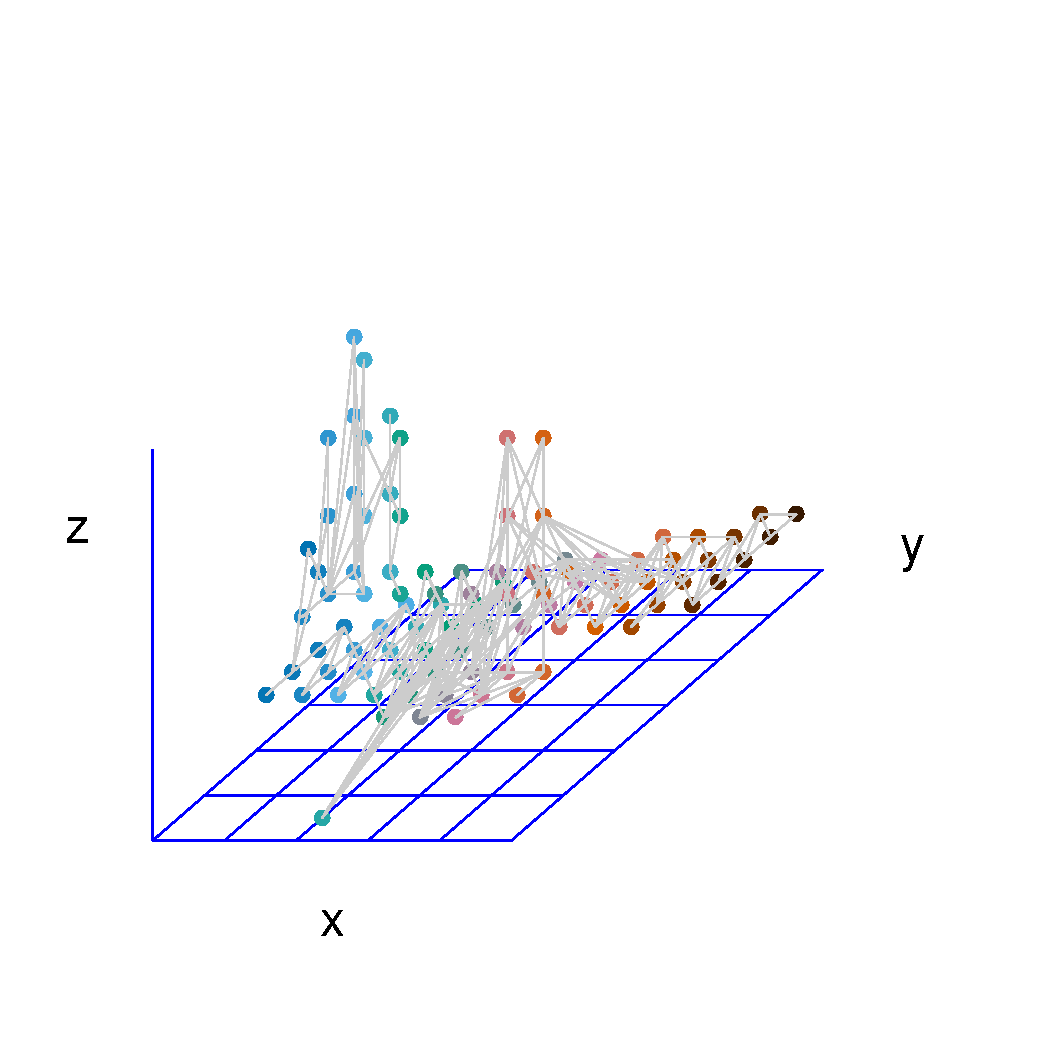
\includegraphics[width=3in]{../Figure/intro.pdf}	
	\label{fig:intro}
	\caption{You can embed each subject (node) connected via edges upon Euclidean space, e.g. $xyz$ 3D-space as above, according to their possessing attributes, e.g. physical location; while how to embed subjects from network into Euclidean space is not intuitive, which should consider their distance with respect to network relationship.}
\end{figure}



\subsection*{Problems in adopting  valid distance metric defined over network}

\begin{figure}[H]
	\centering
	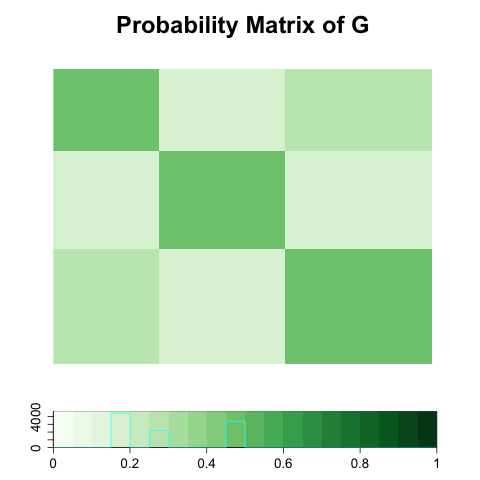
\includegraphics[width=1.5in]{../Figure/pmat.png}
	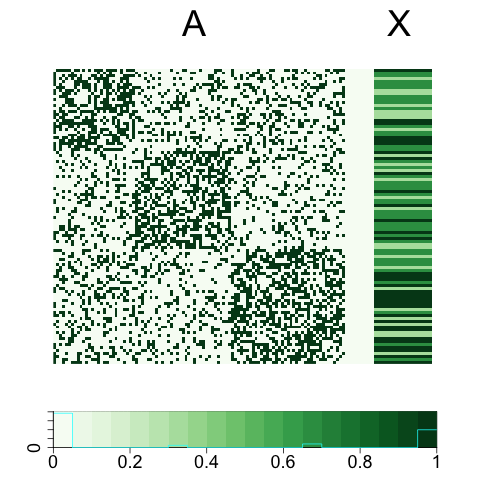
\includegraphics[width=1.5in]{../Figure/Amat.png}
	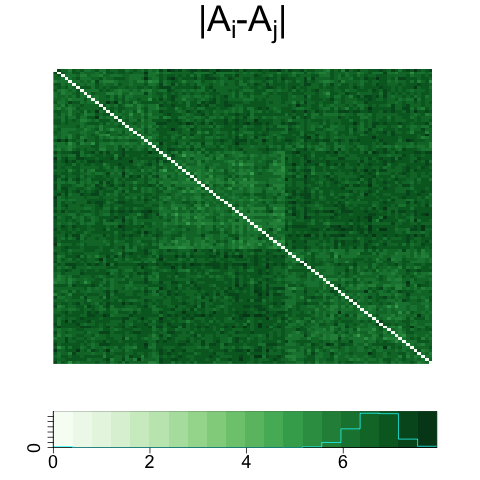
\includegraphics[width=1.5in]{../Figure/distA.png}
	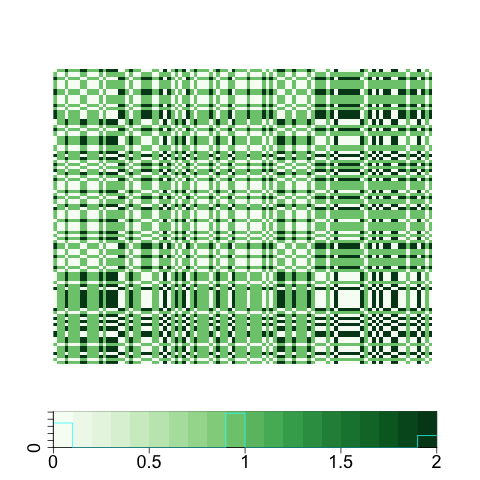
\includegraphics[width=1.5in]{../Figure/distX.png}
	\caption{Assume that a set of edges $\{ A \}$ follow certain stochastic block model, also depending on the distribution function of nodal attributes $X$ (a), then with some amount of noise we have a realized adjacency matrix and a set of attribute outcomes (b) of which Euclidean distances (c $\&$ d) are constructed to be possibly used in standard distance-based independence test.}
	\label{fig:matrics}
\end{figure}	

\subsection*{introduce a family of network distance matrices} 

\begin{figure}[H]
	\centering
	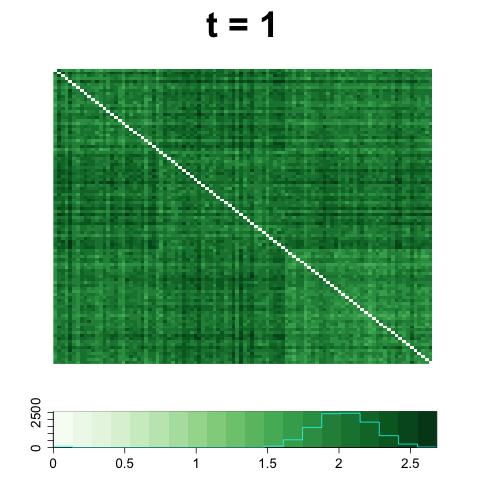
\includegraphics[width=1.5in]{../Figure/Dx1.png}
	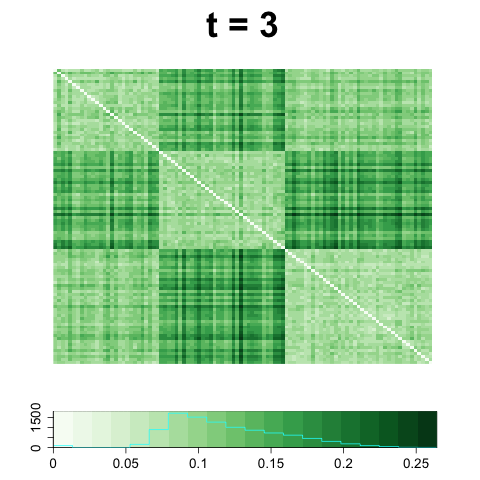
\includegraphics[width=1.5in]{../Figure/Dx3.png}
	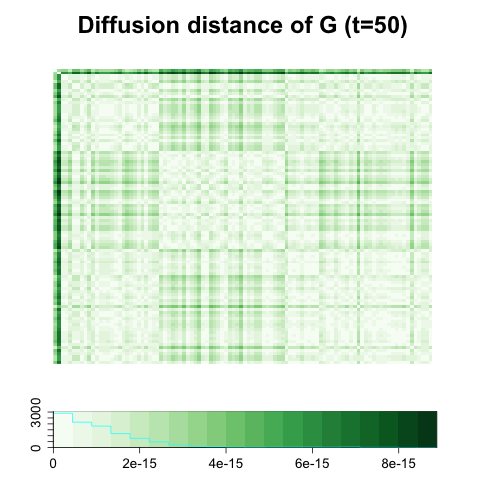
\includegraphics[width=1.5in]{../Figure/Dx50.png}
	\label{fig:diffusions}
	\caption{\textit{Diffusion matrix}, as a proposed alternative for Euclidean distance of $A$, provides one-parameter family of network-based distance where at early stage, e.g. at $t=1$, distance matrix is very similar to Euclidean distance of $A$ but as time goes by the pattern shown in the distance matrix changes, and our optimal time point $t^{*}$ choose the diffusion time when diffusion distance matrix exhibits most dependence to distance matrix of $\mathbf{X}$.}
\end{figure}	


\subsection*{ Empirical power of Oracle MGC/Sample MGC}

\begin{figure}[H]
	\centering
	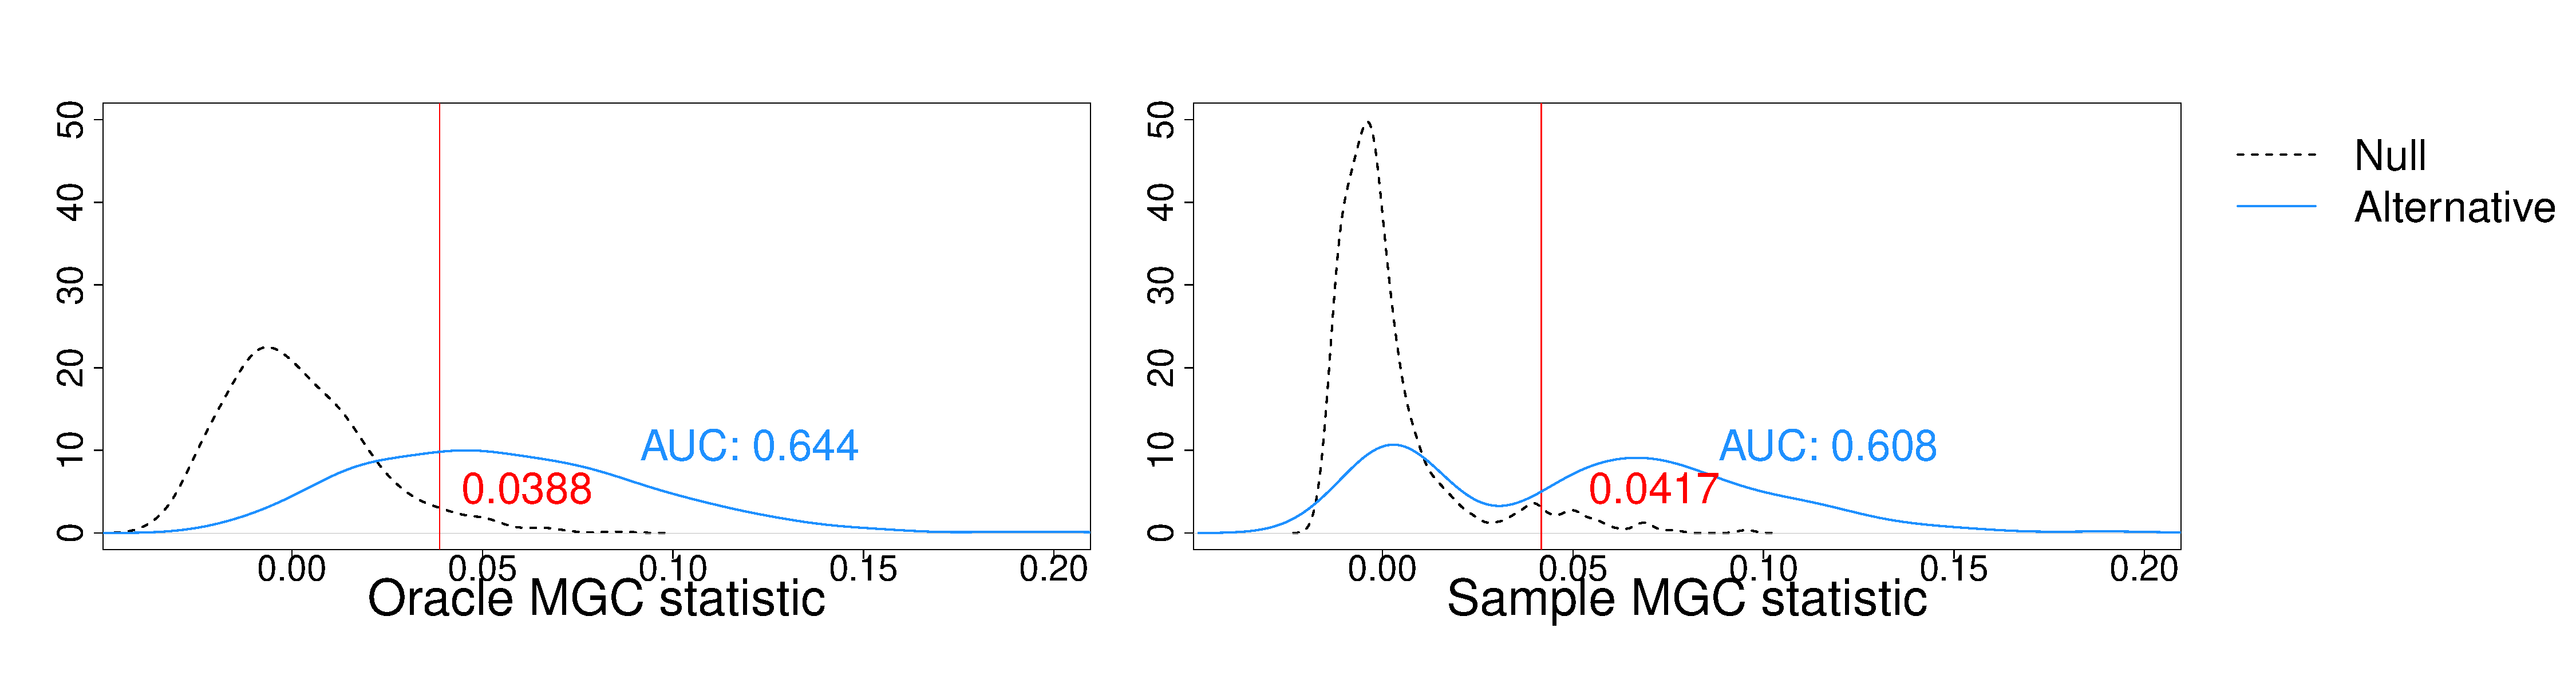
\includegraphics[width=6in]{../Figure/density.pdf}
	\caption{In the left panel we have empirical Null distribution of \texttt{Oracle MGC} illustrated by dotted line of which 95$\%$ sample quantile determines testing power of \texttt{Oracle MGC} by calculating area under the curve (AUC) of the empirical distribution under alternative beyond that quantile, and AUC of \texttt{Oracle MGC} (0.644) looks similar to that of \texttt{Sample MGC} (0.608), as presented in the right panel, even though the shape of its distributions under null and alternative look different, which supports the use of \texttt{Sample MGC} as a substitute for \texttt{Oracle MGC} in real data.}
	\label{fig:density}
\end{figure}	
 
 \newpage
\subsection*{Simplest Stochastic Block Model}
 
\begin{figure}[h]
	\centering
	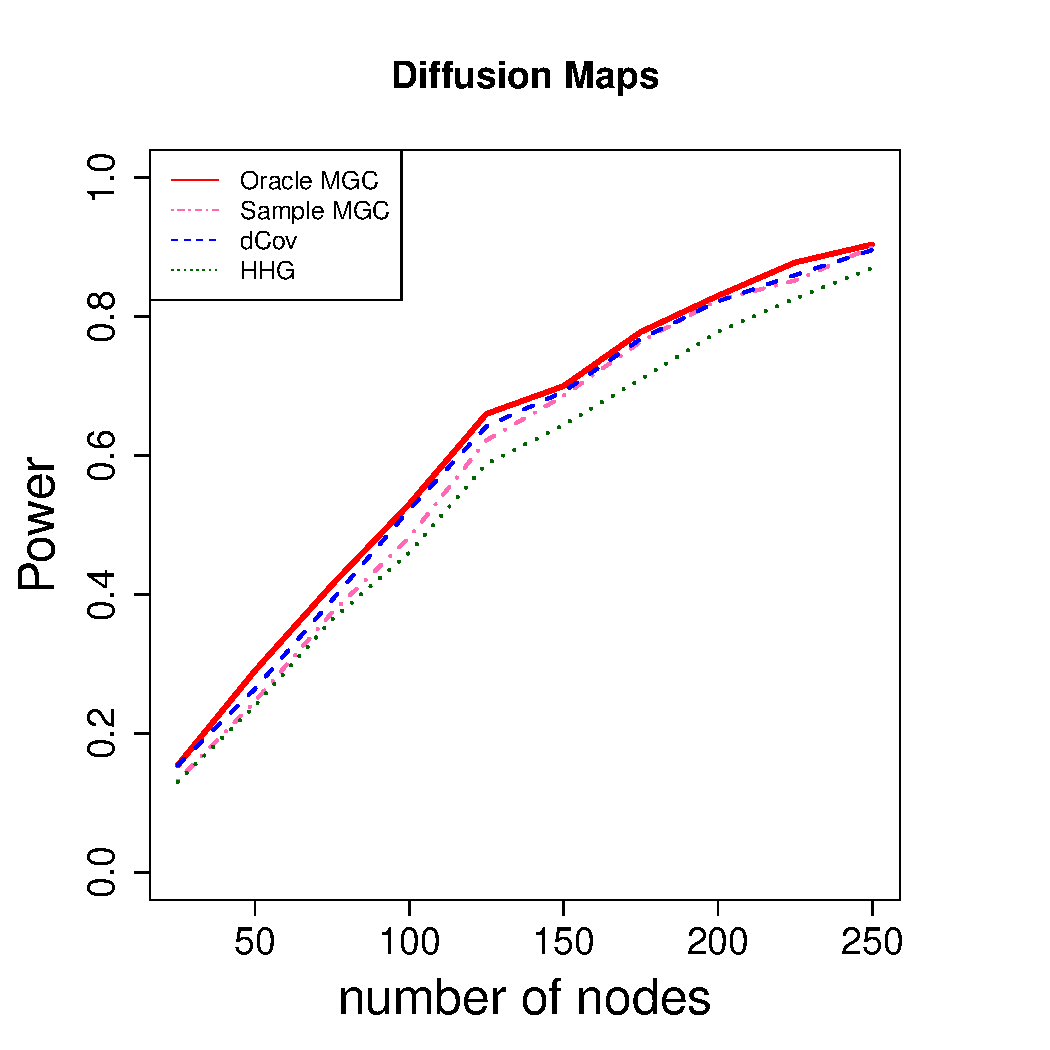
\includegraphics[width=6in]{../Figure/twoSBM.pdf}
	\caption{Above three figures are showing power of network independence test under two block SBM using diffusion maps, adjacency matrix, and estimated latent position as a network distance measure where power of \texttt{MGC} and global distance-based tests (\texttt{dCov, HHG}) are similar in each case and they are doing as good as model-based \texttt{FH} tests under latent factor metrics but still overall power under diffusion maps is the highest.}
	\label{fig:twoSBM}

\end{figure}

\subsection*{Highest power of MGC under diffusion maps}

\begin{SCfigure}[][h]
	\centering
	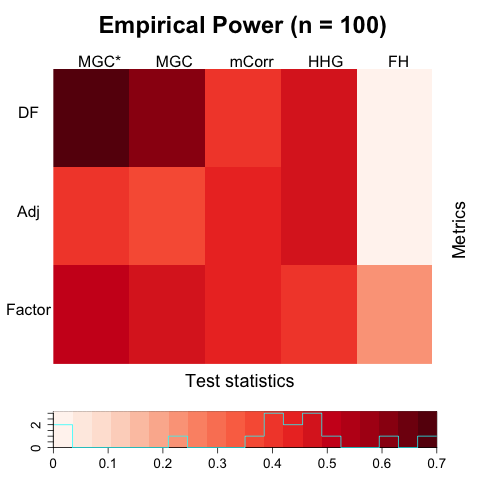
\includegraphics[width=3in]{../Figure/ThreeSBM_results.png}
	\caption{This power heatmap demonstrate superior power of \texttt{Oracle MGC}(MGC*) or \texttt{Sample MGC} (MGC) under diffusion distance matrix under three SBM, compared to adjacency matrix distance or latent factor distance where four distance-based tests show similar power whereas \texttt{FH} test results much less power than the others.}
	\label{fig:threeSBM}
\end{SCfigure}


\newpage
\subsection*{Superiority of the proposed method under non-linear dependency}

\begin{figure}[H]
	\centering
	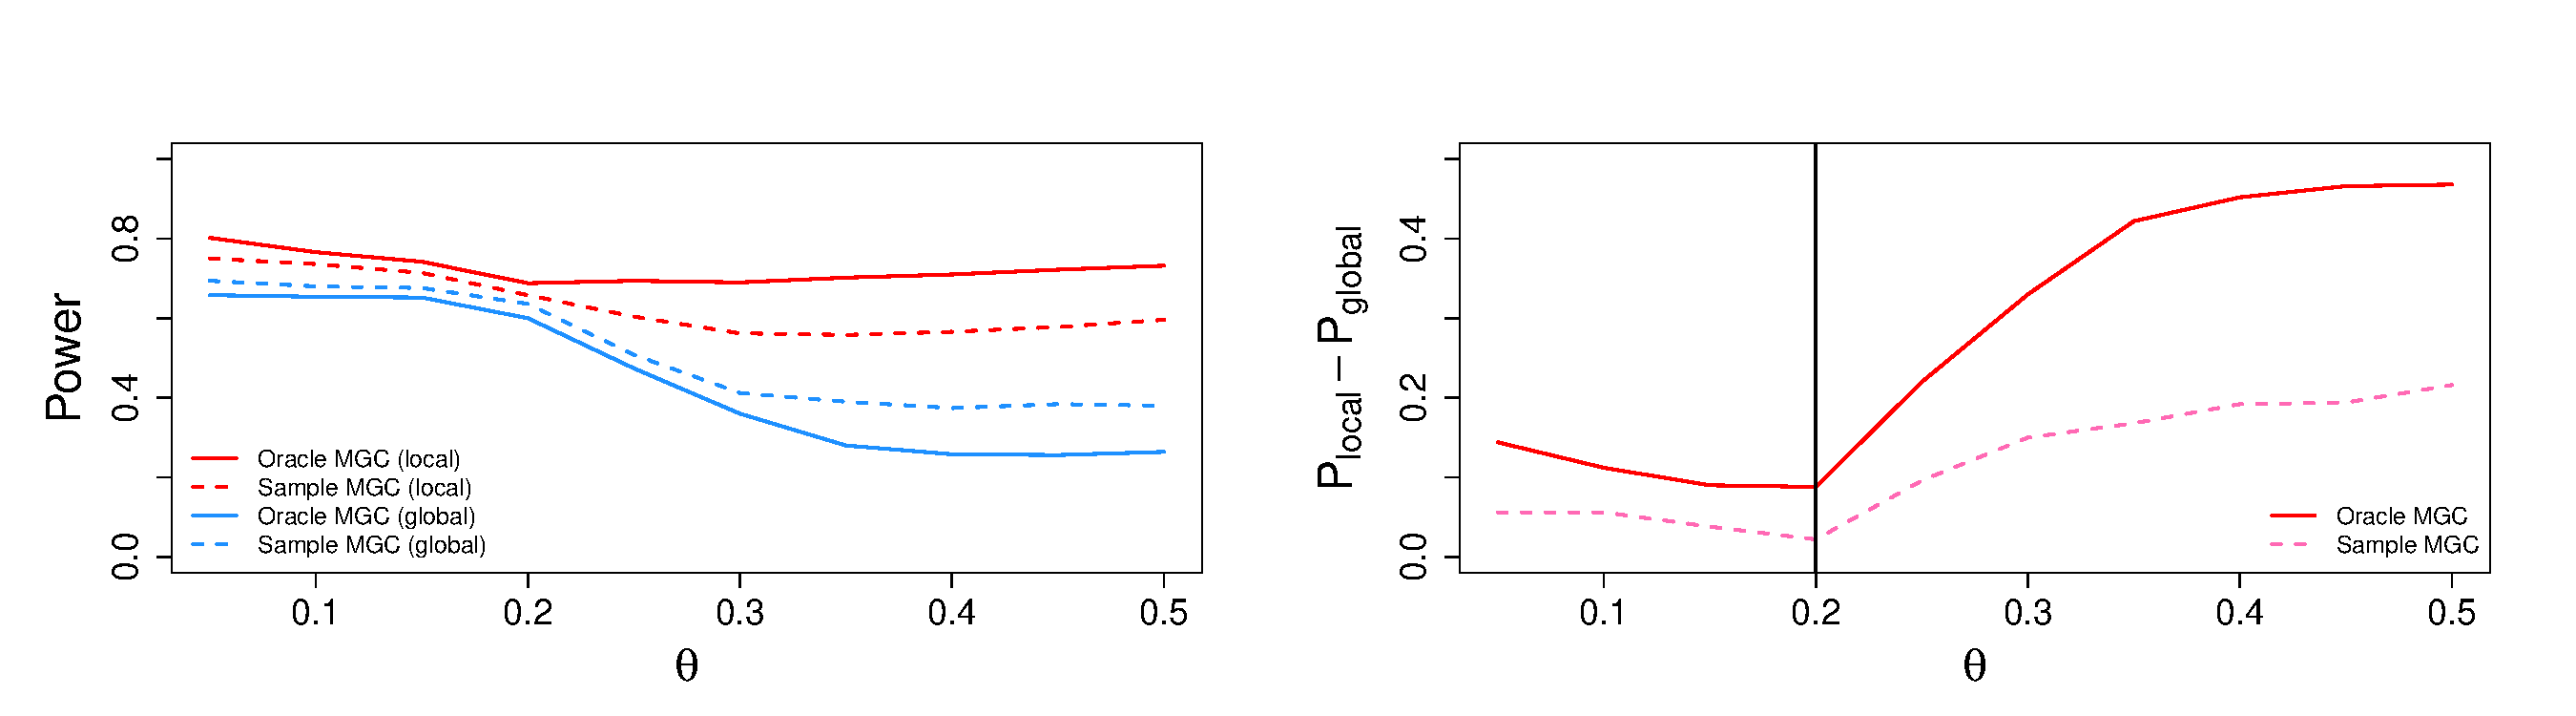
\includegraphics[width=6in]{../Figure/powerplot.pdf}
	\caption{X-axis of $\theta$ controls the existence/amount of non-linear dependency and in this particular case non-linearity exists when $\theta > 0.2$ and gets larger as it increases, and you can see the discrepancy in power between global and local scale tests also gets larger accordingly, mostly due to decreasing power of global test but relatively stable power of \texttt{MGC} under non-linear dependency as presented in the left panel.}
	\label{fig:powerplot}
\end{figure}

\subsection*{Degree-corrected SBM with increased variability in node distribution}	

\begin{figure}[H]
	\centering
	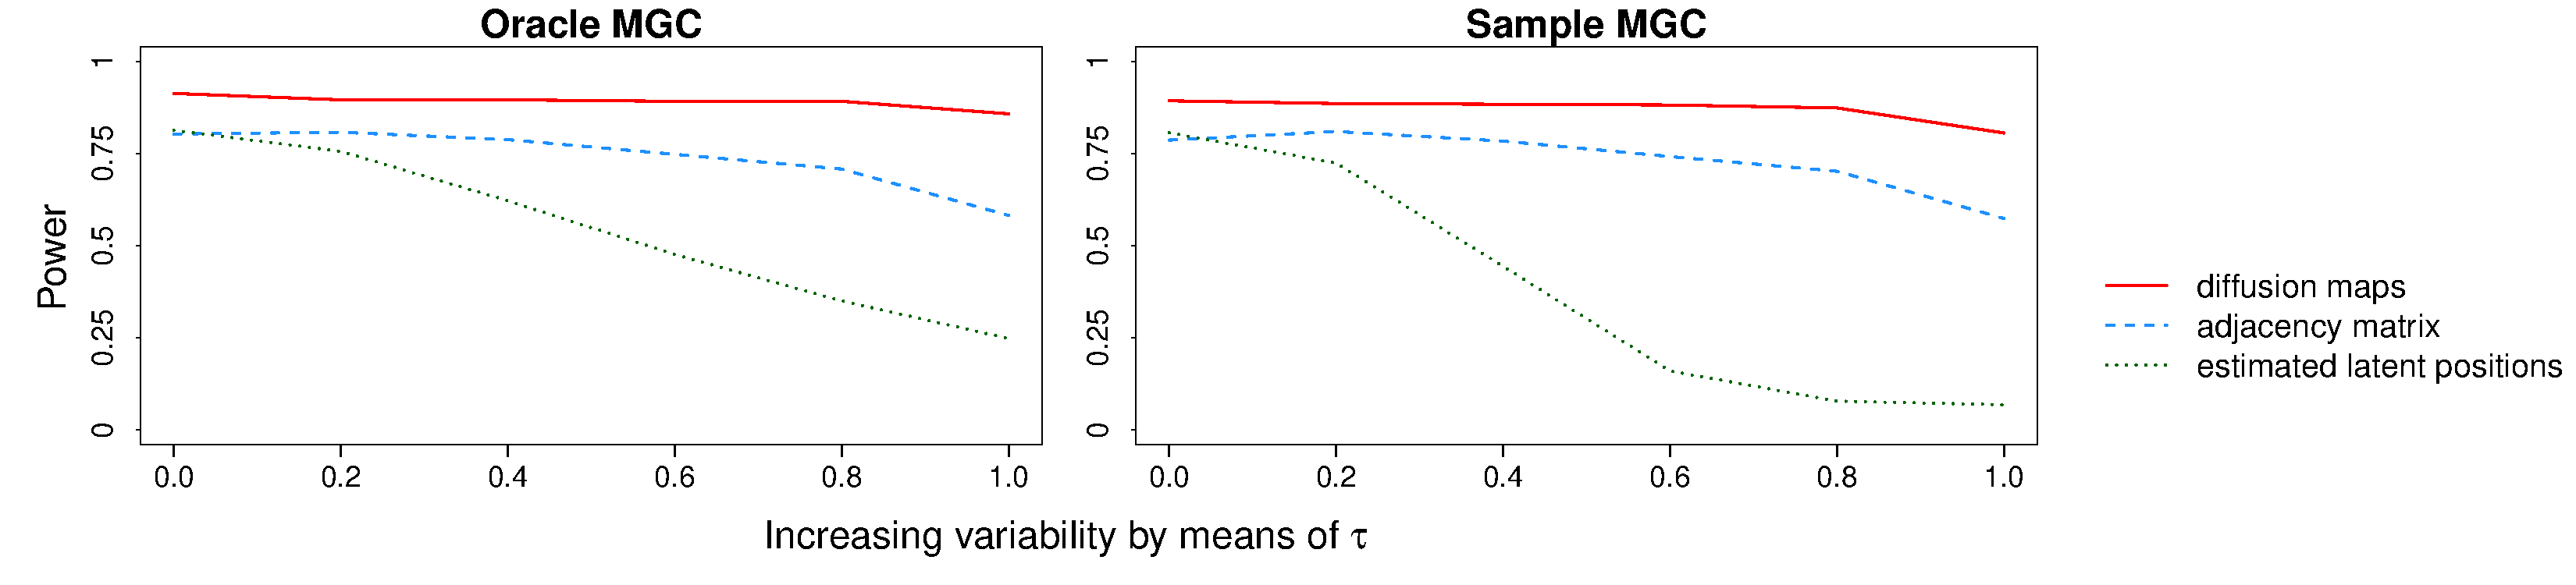
\includegraphics[width=6in]{../Figure/powerplot_var.pdf}
	\caption{In degree-corrected SBM where the variability in degree distribution increases as $\tau$ increases, power of diffusion maps are more likely to be robust against increasing variability compared to adjacency matrix and latent positions.}
	\label{fig:dcSBM}
\end{figure}	

\textbf{Increasing variance in DCSBM}
\begin{equation}
\label{eq:dcVariance}
\begin{gathered}
\begin{aligned}
& \theta_{i} \overset{i.i.d}{\sim} Uniform(1 - \tau, 1 + \tau), i = 1, \ldots, n; \quad \tau = 0, 0.2, \ldots, 1\\ 
& A_{ij} | \mathbf{Z}, \mathbf{\theta}   \overset{i.i.d}{\sim}   f_{A|Z, \theta}(a_{ij} | z_{i}, z_{j}, \theta_{i}, \theta_{j}) \stackrel{d}{=} Bern(0.2 \cdot \theta_{i}\theta_{j}) I ( |z_{i} - z_{j}| = 0 ) \\ & \quad \quad + Bern(0.05 \cdot \theta_{i} \theta_{j} ) I(|z_{i} - z_{j}| = 1), \quad i,j=1, \ldots, n; i < j. 
\end{aligned}
\end{gathered}
\end{equation}

\subsection*{Validity of the method even under competitor's model}

\begin{figure}[H]
	\centering
	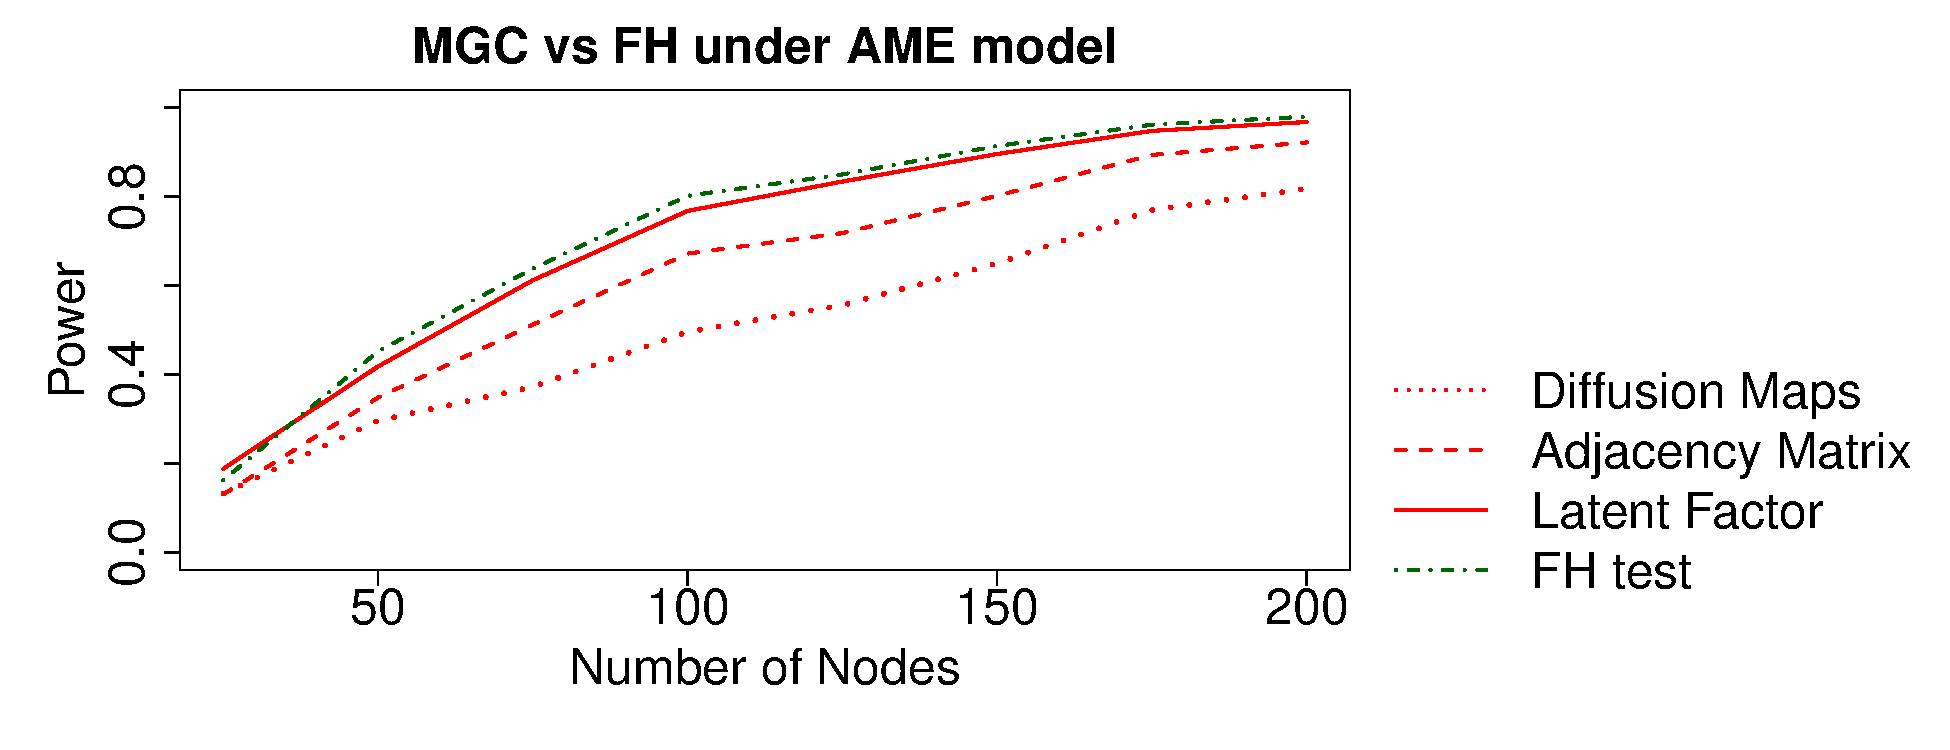
\includegraphics[width=6in]{../Figure/ame_part.pdf}
	\caption{Even under additive and multiplicative model which favors estimated latent position metrics, \texttt{MGC} lost some power when using diffusion maps and adjacency matrix but \texttt{MGC} does as good as \texttt{FH} tests under latent factor metrics, which supports excellent ability of \texttt{MGC} in diverse, nearly true network metrics.}
	\label{fig:ame}
\end{figure}	


\subsection*{Node Contribution}

\begin{SCfigure}[][h]
	\centering
	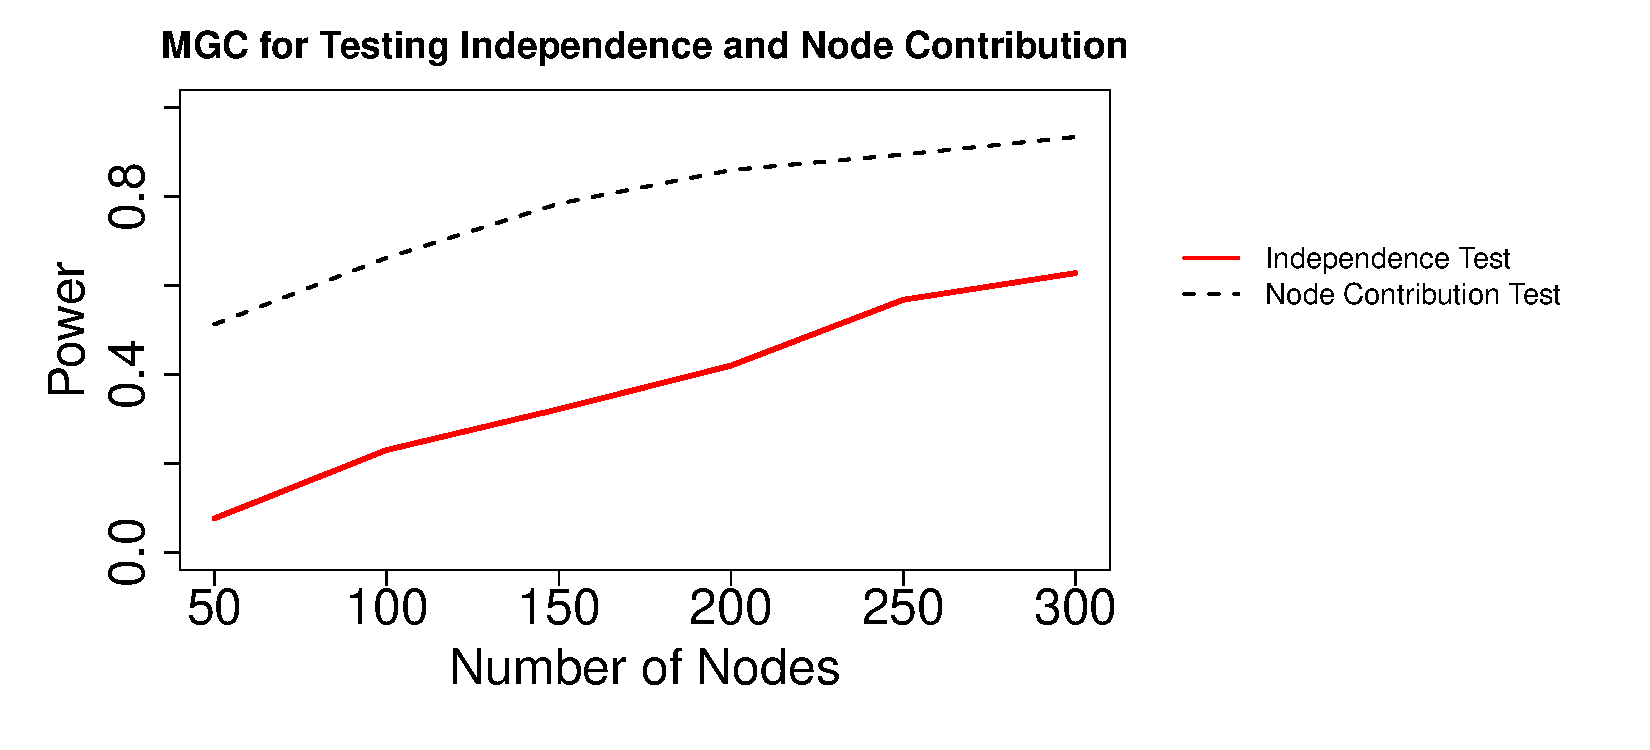
\includegraphics[width=4in]{../Figure/nodecontri.pdf}
	\caption{This plot describes both power of \texttt{MGC} and the rate of correctly-ranked node contribution increase as the number of nodes increases when only half of the nodes for each simulation actually are set to contribute to the independence test, which validates the use of node contribution measure in independence test.}
	\label{fig:contribution}
\end{SCfigure}


\subsection*{Political Network}

\begin{figure}[H]
	\centering
	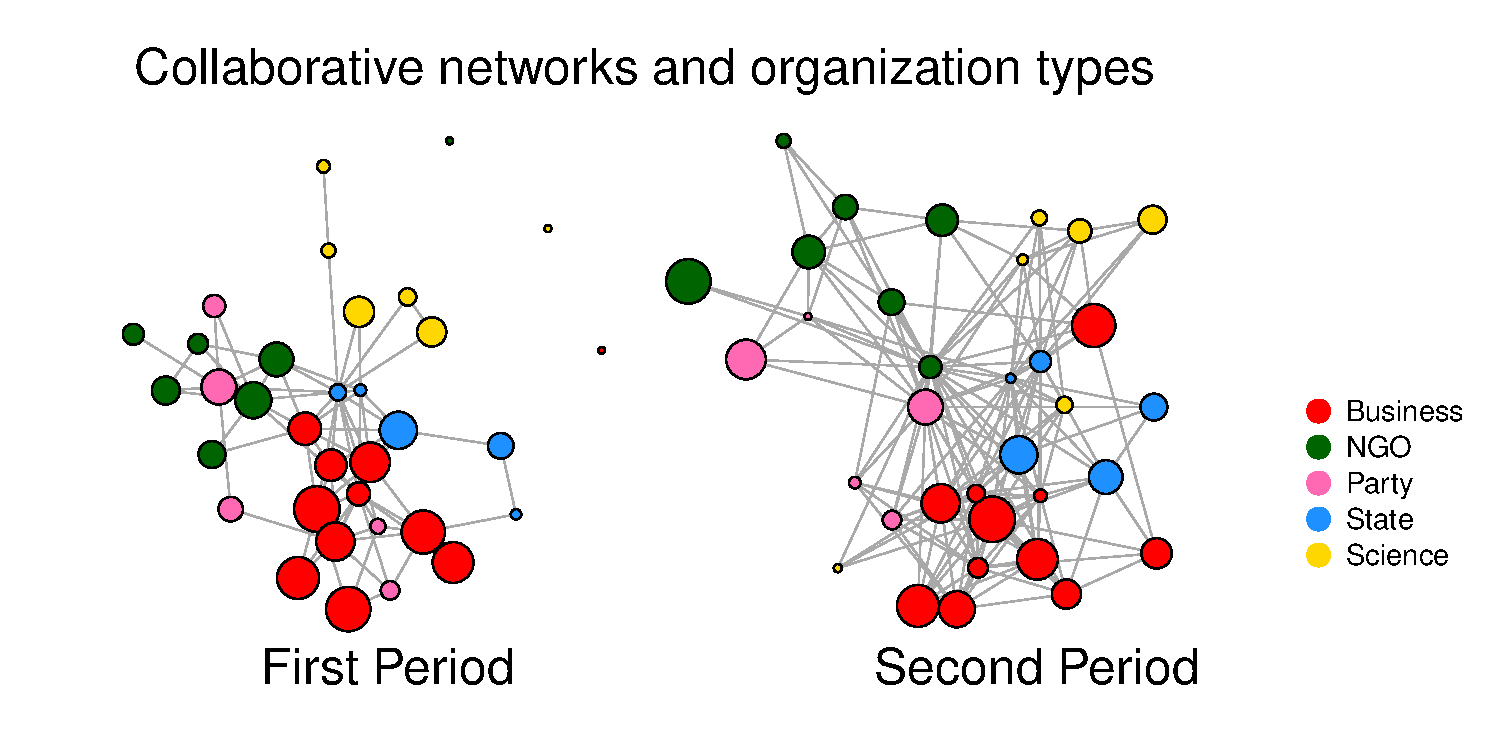
\includegraphics[width=6in]{../Figure/two_politics.pdf}
	\caption{Both networks depict the collaboration network  during the two time periods  comprised of five types of political organizations of which node size is proportional to the rank in terms of contribution to the network independence test.}
	\label{fig:politics}
\end{figure}





\end{document}